\documentclass[pdf,ps2pdf,12pt,report]{SANDreport}
\usepackage{pslatex}
\usepackage{mathptmx}	% Use the Postscript Times font
\usepackage[FIGBOTCAP,normal,bf,tight]{subfigure}
\usepackage[dvips,light,first,bottomafter]{draftcopy}
\draftcopyName{Sample, contains no OUO}{70}

% set tolerance for large spaces between words (affects hyphen)
\tolerance=10000
\vbadness=10000
\hbadness=10000

% PACKAGES ---------------------------------------------------------------
\usepackage{fullpage}
\usepackage{subfigure}
\usepackage{amsfonts}
\usepackage[centertags]{amsmath}
\usepackage{amsthm}
\usepackage{graphicx}
\usepackage{subfigure}
\usepackage{bbm}
\usepackage{url}
\usepackage{color}
\usepackage{algorithm}
\usepackage{algorithmic}
\usepackage{framed}

% THEOREMS ---------------------------------------------------------------
\theoremstyle{plain}
\newtheorem{thm}{Theorem}[section]
\newtheorem{cor}[thm]{Corollary}
\newtheorem{lem}[thm]{Lemma}
\newtheorem{prop}[thm]{Proposition}
\theoremstyle{definition}
\newtheorem{defn}{Definition}[section]
\theoremstyle{remark}
\newtheorem{rem}{Remark}[section]
\numberwithin{equation}{section}
\renewcommand{\theequation}{\thesection.\arabic{equation}}
\renewcommand{\theenumi}{\Roman{enumi}}

% Change section numbering to remove chapter
\renewcommand{\thesection}{\arabic{section}}

% DEFINITIONS ------------------------------------------------------------
%\newcommand{\norm}[1]{\left\Vert#1\right\Vert}
%\newcommand{\abs}[1]{\left\vert#1\right\vert}

% DEFINITIONS ------------------------------------------------------------
\newcommand{\CMPLX}{\ensuremath{\mathbb{C}}}
\newcommand{\REAL}{\ensuremath{\mathbb{R}}}
\newcommand{\ran}{\ensuremath{\mathcal{R}}}
\newcommand{\bdu}{\ensuremath{\mbox{\textbf{u}}}}
\newcommand{\bdx}{\ensuremath{\mbox{\textbf{x}}}}
\newcommand{\bdf}{\ensuremath{\mbox{\textbf{f}}}}
\newcommand{\bdb}{\ensuremath{\mbox{\textbf{b}}}}
\newcommand{\bdy}{\ensuremath{\mbox{\textbf{y}}}}
\newcommand{\bdC}{\ensuremath{\mbox{\textbf{C}}}}
\newcommand{\bdv}{\ensuremath{\mbox{\textbf{v}}}}
\newcommand{\bdzero}{\ensuremath{\mbox{\textbf{0}}}}
\newcommand{\bdeta}{\ensuremath{\mbox{\boldmath$\eta$}}}
\newcommand{\bdxi}{\ensuremath{\mbox{\boldmath$\xi$}}}
\newcommand{\goodgap}{\hspace{\subfigcapskip}}
\def\argmin{\mathop{\rm arg\,min}}
\newcommand{\norm}[1]{\left\Vert#1\right\Vert}
\newcommand{\abs}[1]{\left\vert#1\right\vert}

\newenvironment{packed_itemize}{
\begin{itemize}
  \setlength{\itemsep}{1pt}
  \setlength{\parskip}{0pt}
  \setlength{\parsep}{0pt}
}{\end{itemize}}


% MACROS -----------------------------------------------------------
\newcommand{\comment}[1]{} % makes its argument disappear
% <<< Color >>>
\newcommand\MLP[1]{\textcolor{blue}{[MLP: #1]}}
%%% ----------------------------------------------------------------------


% If you want to relax some of the SAND98-0730 requirements, use the "relax"
% option. It adds spaces and boldface in the table of contents, and does not
% force the page layout sizes.
% e.g. \documentclass[relax,12pt]{SANDreport}
%
% You can also use the "strict" option, which applies even more of the
% SAND98-0730 guidelines. It gets rid of section numbers which are often
% useful; e.g. \documentclass[strict]{SANDreport}



% ---------------------------------------------------------------------------- %
%
% Set the title, author, and date
%
    \title{\emph{Peridigm} Summary Report:\\Lessons Learned in Development with Agile Components}

    \author{Michael Parks, David Littlewood, Andy Salinger, and John Mitchell \\
	  Sandia National Laboratories\\
	  P.O. Box 5800\\
	  Albuquerque, NM 87185 \\
	 }

    % There is a "Printed" date on the title page of a SAND report, so
    % the generic \date should generally be empty.
    \date{}


% ---------------------------------------------------------------------------- %
% Set some things we need for SAND reports. These are mandatory
%
\SANDnum{SAND2011-xxxx}
\SANDprintDate{September 2011}
%\SANDrePrintDate{January 2006}
%\SANDrePrintDate{February 2006}
%\SANDrePrintDate{March 2006}
\SANDauthor{Michael Parks, David Littlewood, Andy Salinger, and John Mitchell }


% ---------------------------------------------------------------------------- %
% Include the markings required for your SAND report. The default is "Unlimited
% Release". You may have to edit the file included here, or create your own
% (see the examples provided).
%
% \include{MarkUR} % Not needed for unlimted release reports


% ---------------------------------------------------------------------------- %
% The following definition does not have a default value and will not
% print anything, if not defined
%
%\SANDsupersed{SAND1901-0001}{January 1901}


% ---------------------------------------------------------------------------- %
%
% Start the document
%
\begin{document}
    \maketitle

    % ------------------------------------------------------------------------ %
    % An Abstract is required for SAND reports
    %
\begin{abstract}
This report details efforts to deploy \emph{Agile Components} for rapid development of a peridynamics code, \emph{Peridigm}.  The goal of Agile Components is to enable the efficient development of production-quality software by providing a well-defined, unifying interface to a powerful set of component-based software.  Specifically, Agile Components facilitate interoperability among packages within the \emph{Trilinos Project}, including data management, time integration, uncertainty quantification, and optimization. Development of the \emph{Peridigm} code served as a testbed for Agile Components and resulted in a number of recommendations for future development.  Agile Components successfully enabled rapid integration of \emph{Trilinos} packages into \emph{Peridigm}.  A cost of this approach, however, was a set of restrictions on \emph{Peridigm}'s architecture which impacted the ability to track history-dependent material data, dynamically modify the model discretization, and interject user-defined routines into the time integration algorithm.  These restrictions resulted in modifications to the Agile Components approach, as implemented in \emph{Peridigm}, and in a set of recommendations for future Agile Components development.  Specific recommendations include improved handling of material states, a more flexible flow control model, and improved documentation.  A demonstration mini-application, \emph{SimpleODE}, was developed at the onset of this project and is offered as a potential supplement to Agile Components documentation.
\end{abstract}


    % ------------------------------------------------------------------------ %
    % The table of contents and list of figures and tables
    % Comment out \listoffigures and \listoftables if there are no
    % figures or tables. Make sure this starts on an odd numbered page
    %
    \cleardoublepage		% TOC needs to start on an odd page
    \tableofcontents
    \listoffigures
%    \listoftables     % we don't have any tables


    % ---------------------------------------------------------------------- %
    % An optional preface or Foreword
%    \clearpage
%    \chapter*{Preface}
%    \addcontentsline{toc}{chapter}{Preface}



    % ---------------------------------------------------------------------- %
    % An optional executive summary
%    \clearpage
%    \chapter*{Executive Summary}
%    \addcontentsline{toc}{chapter}{Executive Summary}
%This report details efforts to deploy \emph{Agile Components} for rapid development of a peridynamics code, \emph{Peridigm}.  The goal of Agile Components is to enable the efficient development of production-quality software by providing a well-defined, unifying interface to a powerful set of component-based software.  Specifically, Agile Components facilitate interoperability among packages within the \emph{Trilinos Project}, including data management, time integration, uncertainty quantification, and optimization.  Development of the \emph{Peridigm} code served as a testbed for Agile Components and resulted in a number of recommendations for future development.  Agile Components successfully enabled rapid integration of \emph{Trilinos} packages into \emph{Peridigm}.  A cost of this approach, however, was a set of restrictions on \emph{Peridigm}'s architecture which impacted the ability to track history-dependent material data, dynamically modify the model discretization, and interject user-defined routines into the time integration algorithm.  These restrictions resulted in modifications to the Agile Components approach, as implemented in \emph{Peridigm}, and in a set of recommendations for future Agile Components development.  Specific recommendations include improved handling of material states, a more flexible flow control model, and improved documentation.  A demonstration mini-application, \emph{SimpleODE}, was developed at the onset of this project and is offered as a potential supplement to Agile Components documentation.


    % ---------------------------------------------------------------------- %
    % This is where the body of the report begins; usually with an Introduction
    %
    \SANDmain		% Start the main part of the report

\section{Introduction}

The notion that software should be built from prefabricated components has been prominent since the late 1960s. Software components have sometimes been referred to as \emph{software ICs} \cite{Cox:OOP:1991}, with the visionary notion that component-based software can be as impactful to software development as integrated circuit components were to modern electronics. Following in that vein, Agile Components is a strategic effort at Sandia to to enable the efficient development of production-quality software by providing a well-defined, unifying interface to a powerful set of component-based software. 

This report details efforts to test and evaluate the Agile Components methodology by deploying it for the rapid development of a peridynamics code, \emph{Peridigm}. Peridynamics was selected as the driver application because it is unlike the PDE-based finite element models for which Agile Components is most commonly used. Peridynamics is based upon integral equations, not PDEs, and is commonly discretized using a meshfree method, requiring a different computational structure than that of mesh-based finite elements. The \emph{Peridigm} code requires the ability to track history-dependent material data, dynamically modify the model discretization, and interject user-defined routines into the time integration algorithm -- capabilities prior applications had not demanded of Agile Components. These requirements helped to illuminate assumptions made by the interfaces utilized in Agile Components. This provided for a clear identification of the set of ideal target applications for Agile Components, as well as recommendations for modification to Agile Components to broaden their scope and impact.

In \S\ref{sec:ACMeth} we review the Agile Components methodology, including the \emph{ModelEvaluator} interface. We discuss the practical experiences with Agile Components in \S\ref{sec:PracticalACExperience}, discussing the \emph{SimpleODE}, \emph{Albany}, and \emph{Peridigm} codes. In particular, we detail in \S\ref{sec:peridigm} specific issues encountered in deploying Agile Components within Peridigm, including the handling of state within models, history dependence in material models, load rebalance and mesh adaptivity, data distribution, time integration, and control flow. In \S\ref{sec:recommendations} we make specific recommendations to address the development issues we encountered, which we feel will broaden the scope of Agile Components.  

\section{The Agile Components Methodology} \label{sec:ACMeth}

\emph{Agile Components} is a strategic effort at Sandia to maximize both developer efficiency and the impact of our computational science libraries. The intent is to coordinate Sandia software development efforts through a common set of interfaces to better utilize and deliver our computational science capabilities, in particular those tied to the \emph{Trilinos Project}, for the modeling and simulation of physical systems (primarily PDEs). The strategic goals of the Agile Components methodology are:
\begin{packed_itemize}
  \item Enable rapid development of new production codes,
  \item Embed these codes with transformational design, analysis, and decision-support capabilities ({\it e.g.}, embedded uncertainty quantification (UQ), sensitivity analysis, and optimization),
  \item Reduce redundancy.
\end{packed_itemize}

The Agile Components methodology utilizes software components and software quality tools from the \emph{Trilinos Project}, a Sandia effort to develop algorithms and enabling technologies within an object-oriented software framework for the solution of large-scale, complex multi-physics research and engineering problems~\cite{Trilinos-Overview}. Some \emph{Trilinos} capabilities are shown in Figure~\ref{fig:ACCapabilities}.

The Agile Components methodology focuses on delivering capabilities of \emph{Trilinos} software components through a set of well-designed interfaces. As a practical example, a schematic of the \emph{Albany} Agile Components code is shown in Figure~\ref{fig:ACAlbany}, which depicts several of the capabilities from Figure~\ref{fig:ACCapabilities} connected through interfaces.
\begin{figure}[htbp]
  \begin{center}
  \begin{minipage}[b]{0.8\linewidth}
    \centering
    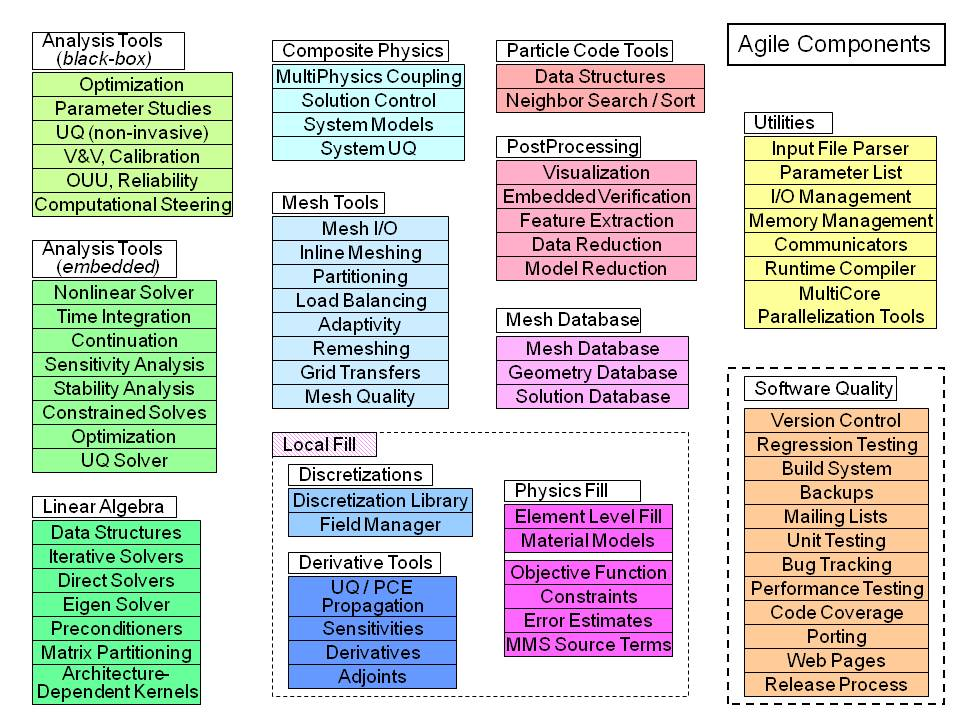
\includegraphics[width=\linewidth]{AgileComponents1}
    \caption{Capabilities delivered by the Agile Components methodology via \emph{Trilinos} components.}
    \label{fig:ACCapabilities}
  \end{minipage}
  \begin{minipage}[b]{0.8\linewidth}
    \centering
    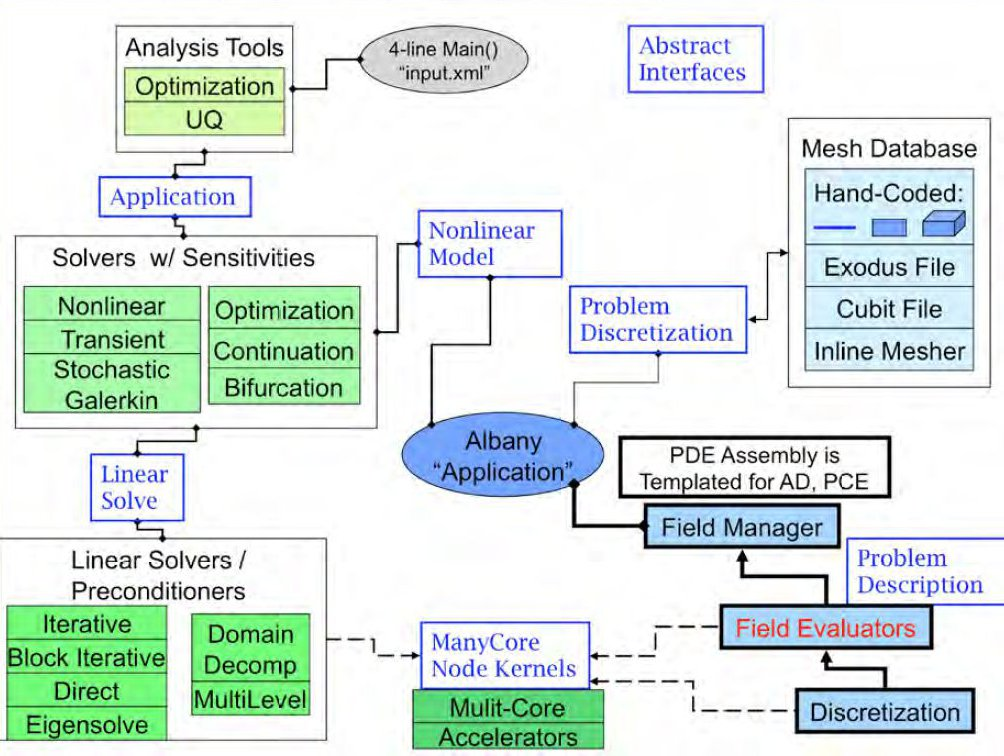
\includegraphics[width=0.7\linewidth]{AgileComponents2}
    \caption{The component-based \emph{Albany} code: A deployment of capabilities from Figure 1 via Agile Components to form a demonstration application.}
    \label{fig:ACAlbany}
  \end{minipage}
  \end{center}
\end{figure}
The design of these interfaces is key to delivering capabilities through Agile Components to an end-user application. Each software component in \emph{Trilinos} implements its own interface, requiring a component-based code to adhere to the different interfaces of each of the \emph{Trilinos} software components it consumes, as depicted in Figure \ref{fig:ACInterfaces1}.  This increases time to deployment, and requires code to be refactored every time a component interface changes.   Figure~\ref{fig:ACInterfaces2} illustrates the Agile Components approach to \emph{Trilinos} solver components; application codes are presented with a single interface with which to consume solver capabilities.  In addition to supplying a unified interface to component functionality, this interface can provide metadata analysis utilities such as embedded UQ, sensitivity analysis, and optimization.  Applications codes adhering to an Agile Components interface receive these additional capabilities without additional burden on the developer.

\begin{rem}
\textbf{The primary roles of Agile Components are to (1) deliver interfaces to software components to facilitate their use, deployment, and adoption, and (2) deliver metadata analysis tools (embedded UQ, sensitivity analysis, optimization, etc.)}
\end{rem}

\begin{figure}[htbp]
  \begin{minipage}[b]{\linewidth}
    \centering
    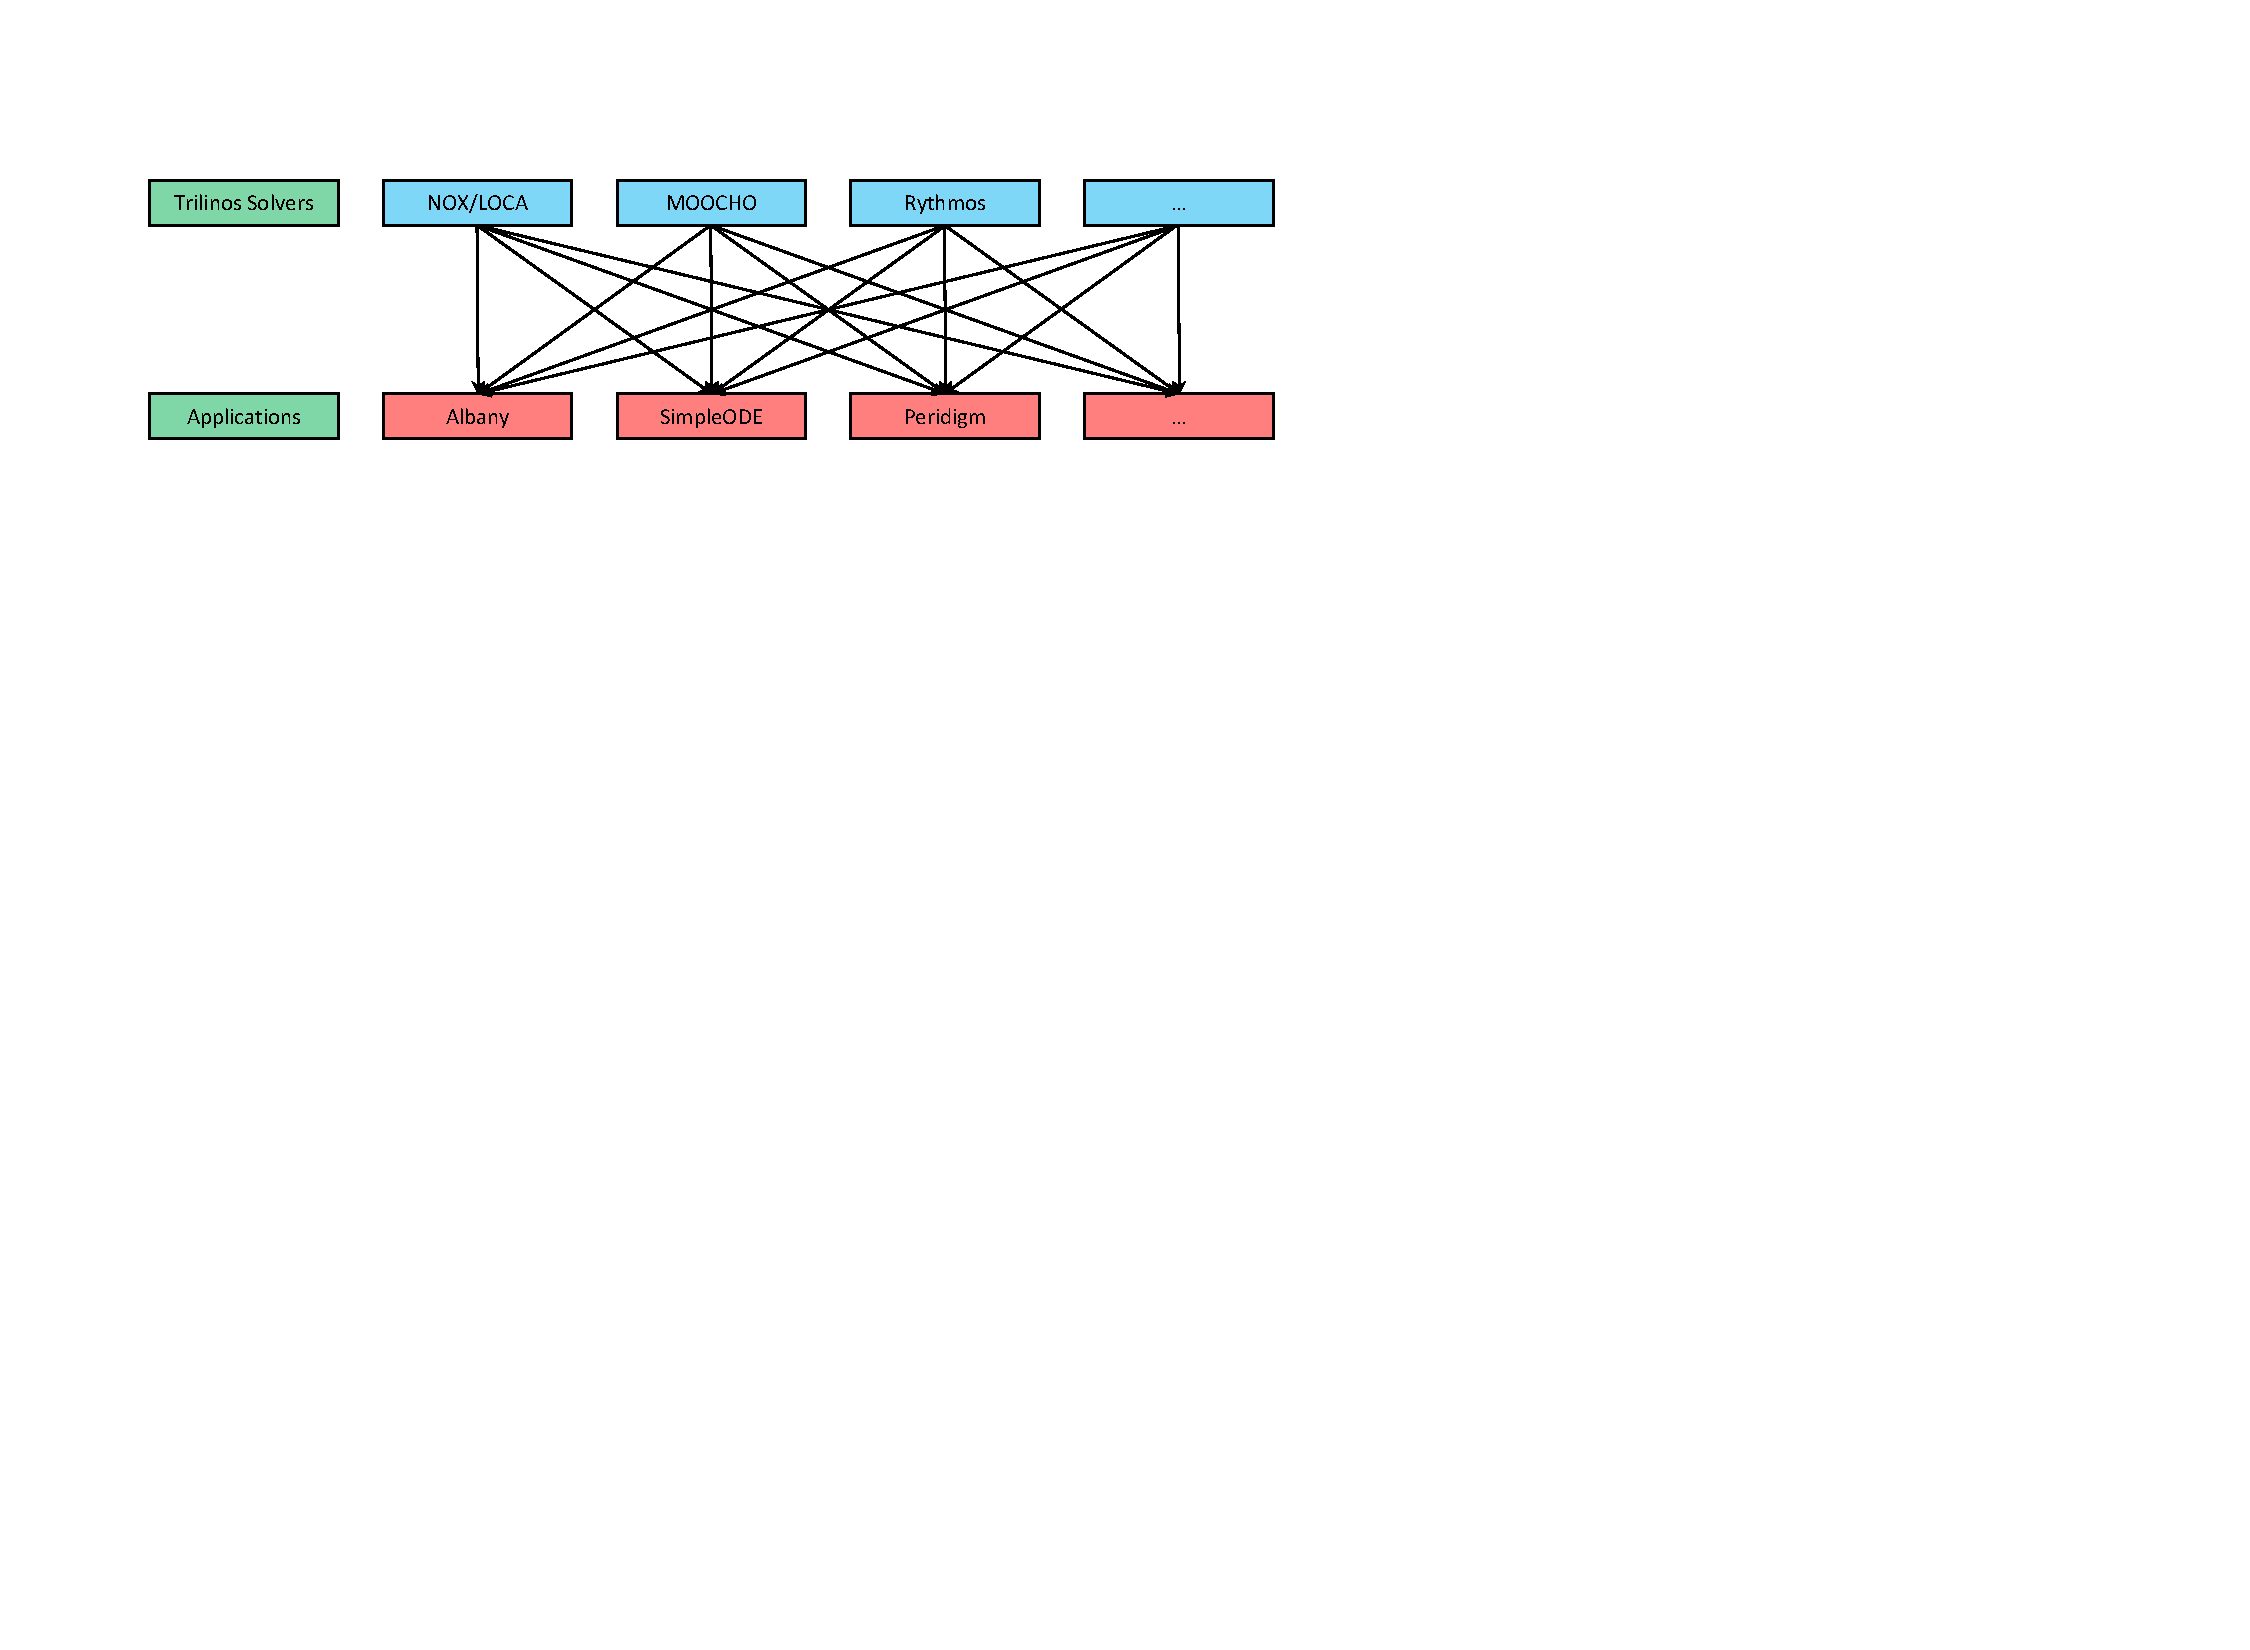
\includegraphics[width=\linewidth]{Interfaces1}
    \caption{Direct interfaces between \emph{Trilinos} components and application codes. Each solver component implements its own interface that must be utilized by the application code.}
    \label{fig:ACInterfaces1}
  \end{minipage}
  \begin{minipage}[b]{\linewidth}
    \centering
    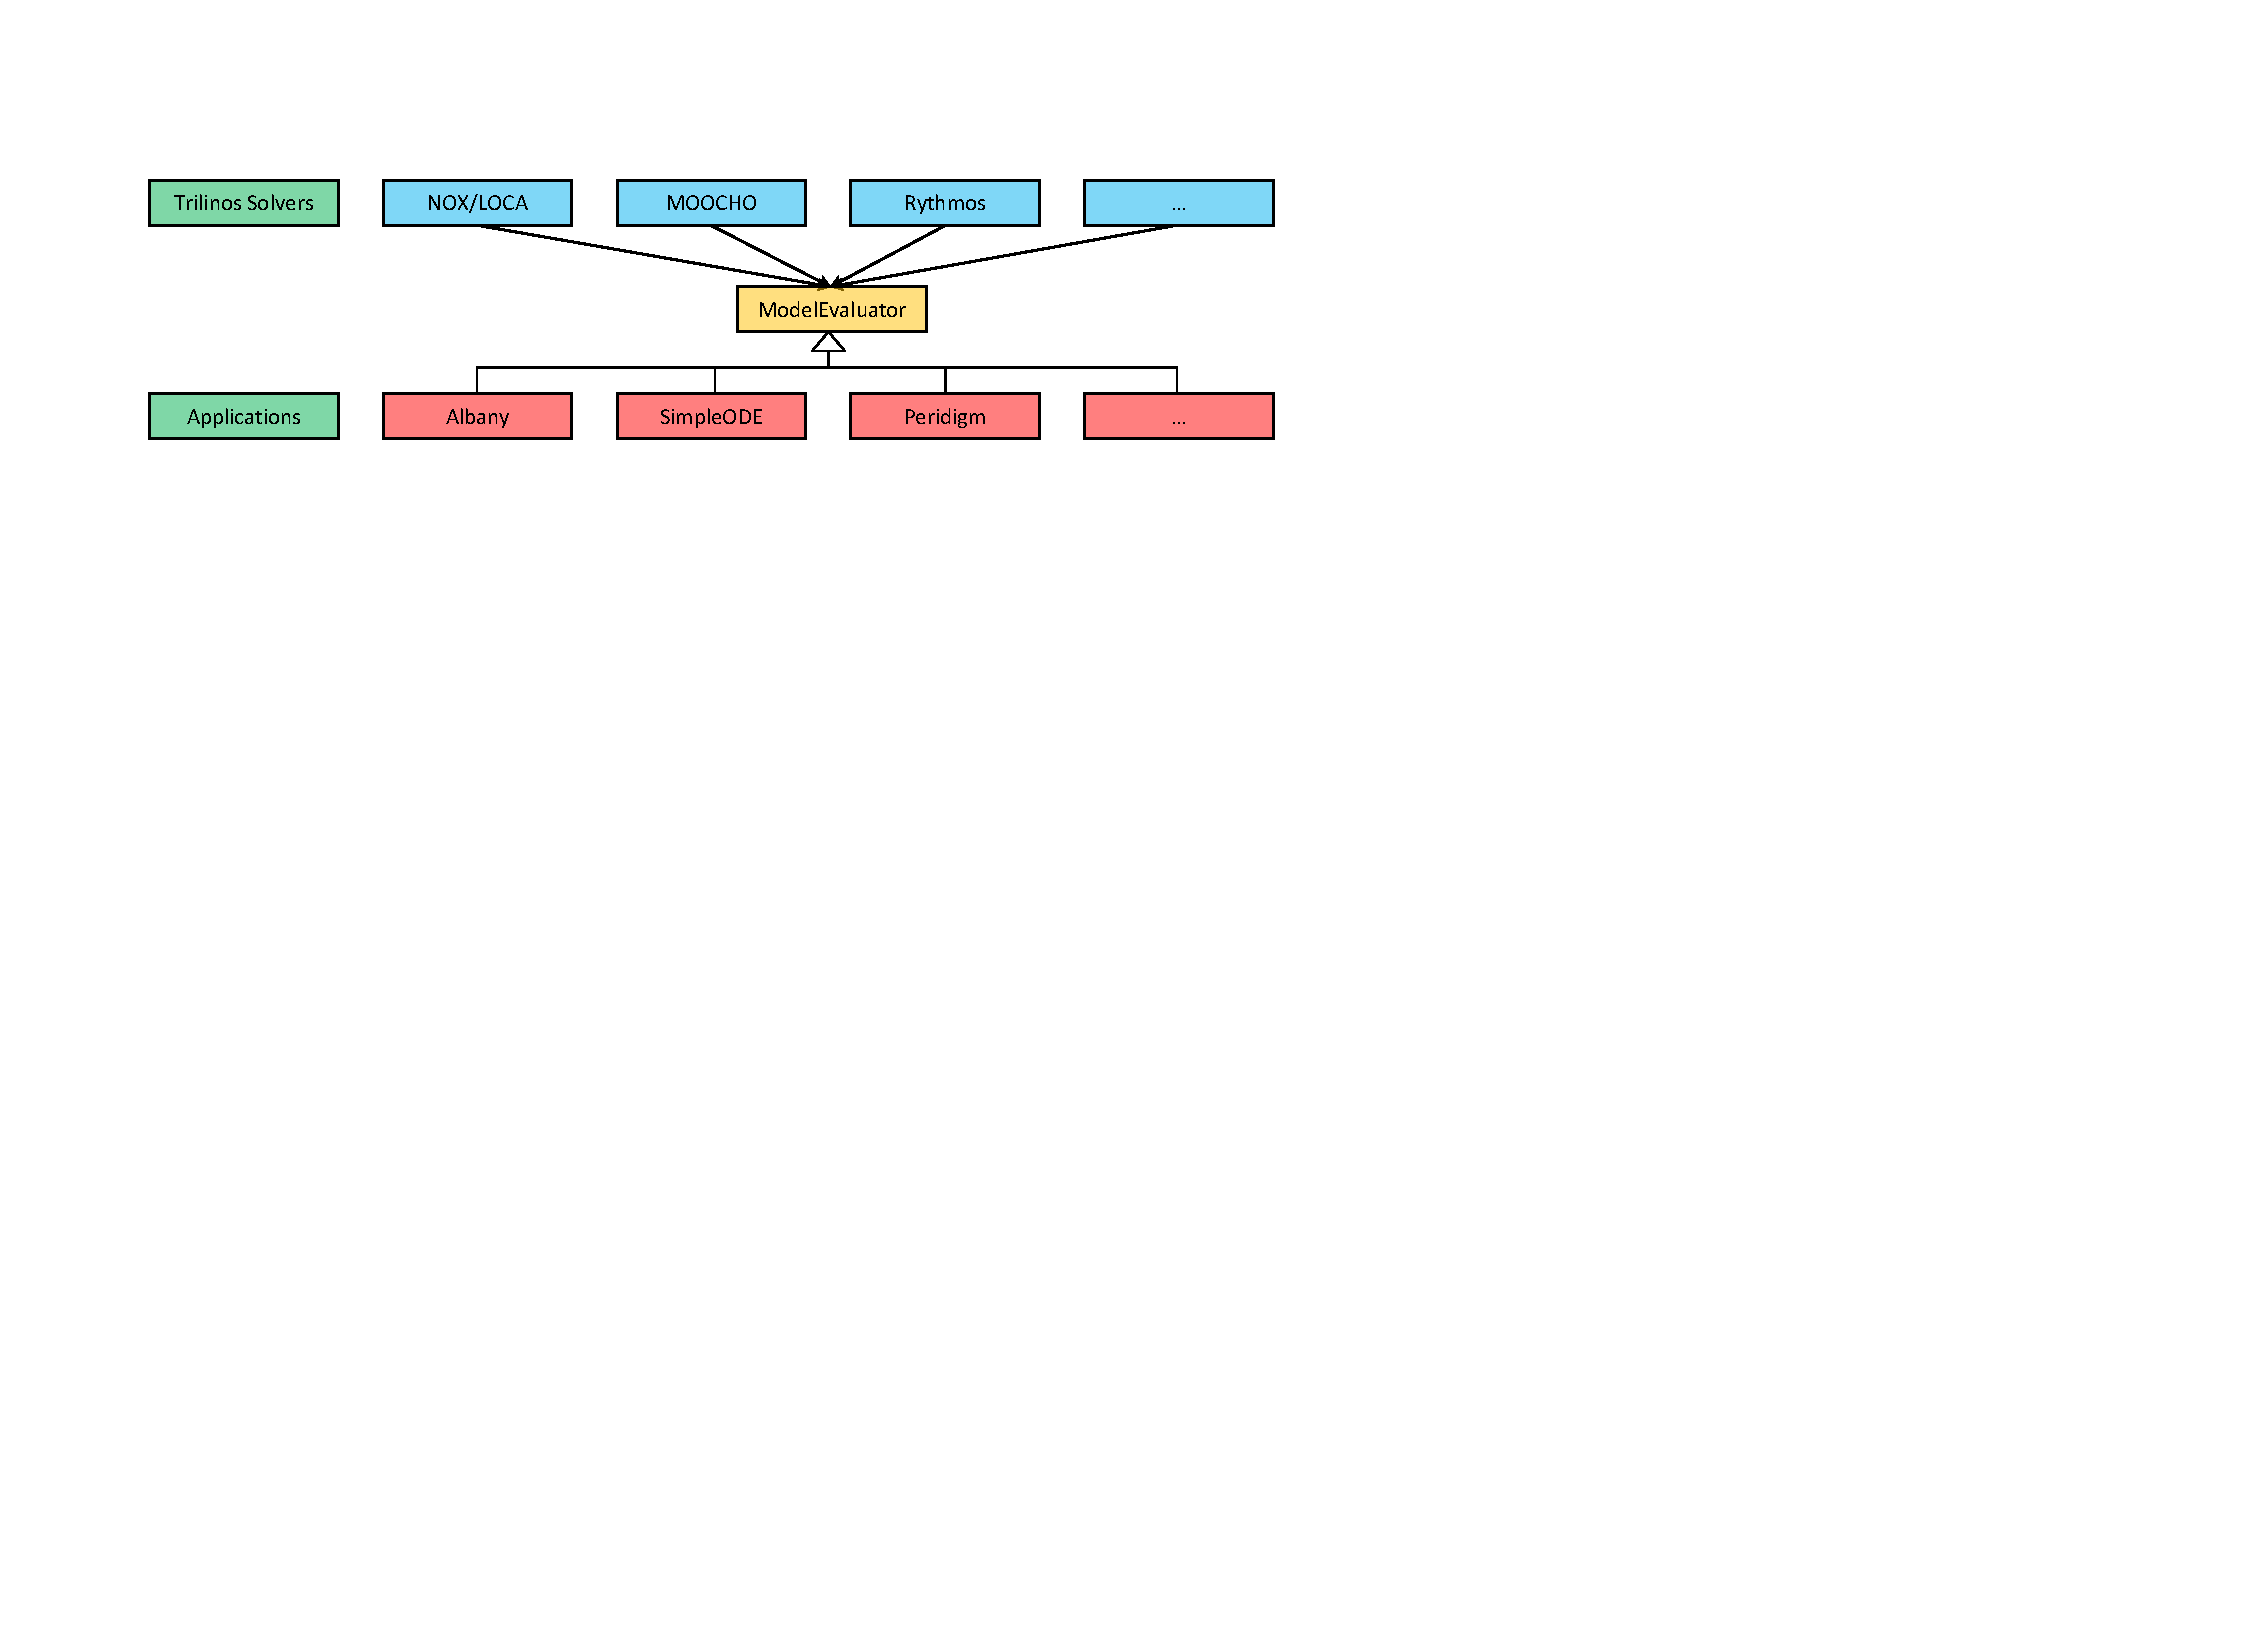
\includegraphics[width=\linewidth]{Interfaces2}
    \caption{\emph{ModelEvaluator} interface between \emph{Trilinos} components and application codes. A common interface facilitates use, deployment, and adoption of solver components.}
    \label{fig:ACInterfaces2}
  \end{minipage}
\end{figure}

\begin{figure}[htbp]
\begin{center}
	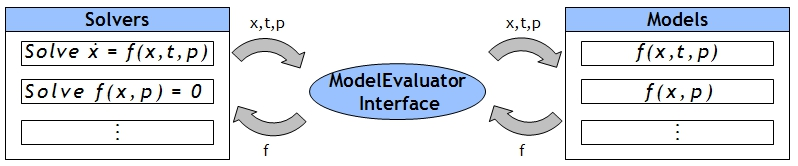
\includegraphics[width=\linewidth]{ModelEvaluatorInterface}
 \end{center}
 \caption{Diagram of the Agile Components \emph{ModelEvaluator} interface.}
\label{fig:ACModelEvaluator}
\end{figure}

\subsection{The Agile Components Interface Paradigm: The \emph{ModelEvaluator} Class}


To achieve the strategic goals of the Agile Components methodology, a set of sufficiently general interfaces is required. This includes interfaces to linear solvers, mesh databases, solver applications, and may include architecture-aware compute kernels. Of central importance to the \emph{Peridigm} application is the \emph{ModelEvaluator}, the abstraction utilized by solver components (such as nonlinear solvers and time integrators) which must be implemented by model developers.

The leftmost column in Figure~\ref{fig:ACModelEvaluator} lists the mathematical problems for which solvers exist within \emph{Trilinos}. These solvers address mathematical problems without specific knowledge of the right-hand-side, $\mathbf{f}$. Model developers provide specific instances of $\mathbf{f}$. The \emph{ModelEvaluator} interface represents a contract between the solver and the model. The \emph{ModelEvaluator} supports the solution of nonlinear equations, stability analysis, explicit first-order ODEs, implicit first-order ODEs, explicit first-order ODE forward sensitivities, implicit first-order ODE forward sensitivities, constrained optimization, unconstrained optimization, and ODE constrained optimization.

\begin{rem} \label{rem:MEContract}
\textbf{The contract enforced by the \emph{ModelEvaluator} assumes that the models $\mathbf{f}$ are stateless, referentially transparent, pure mathematical functions.}
\end{rem}

This is a reasonable assumption, as an optimizer must evaluate a model for many different inputs without regard to the order in which evaluations occur. An important property of pure mathematical functions is that they are \emph{referentially transparent}. A referentially transparent function $\mathbf{f}$ always provides the same output when given the same input, as it contains no state.
\begin{defn} \label{defn:RT}
An expression is referentially transparent if it can be replaced with its value without changing the behavior of a program~\cite{HGVJ:1994:DesignPatterns}.
\end{defn}

%%% ----------------------------------------------------------------------
\section{Practical Experiences with Agile Components} \label{sec:PracticalACExperience}

The Agile Components methodology has been deployed for the development of several application codes, including the multiphysics finite element code \emph{Albany}, the peridynamics code \emph{Peridigm}, and the demonstration mini-application, \emph{SimpleODE}.  An overview of the development process for each of these codes is given below, with an emphasis on the use of \emph{Trilinos} Agile Components.

\begin{rem}
\textbf{Models that fit into the assumptions and implicit contract enforced by the \emph{ModelEvaluator} interface (\emph{cf.} Remark \ref{rem:MEContract}) can naturally and relatively effortlessly utilize this interface for rapid development. Models that violate the assumptions of this interface can not.}
\end{rem}

\subsection{\emph{SimpleODE}, an Agile Components Demonstration MiniApplication} \label{sec:simpleode}

During the course of the development of \emph{Peridigm}, the MiniApp \emph{SimpleODE} was created to demonstrate the use of Agile Components on the simplest problem we could conceive:
\begin{align}
  \dot{x} = -c x, \qquad x(0)=x_0,
\end{align}
with $c>0$ a constant. The principle purpose of \emph{SimpleODE} is to provide a template for other developers wishing to create their own agile component code. Unlike \emph{Albany} (\emph{cf.}~\S\ref{sec:albany}), which is a full-blown Agile Components application, \emph{SimpleODE} contains all of the Agile Components infrastructure without a complex application model to obscure that infrastructure.

The execution control flow of \emph{SimpleODE} is presented in Figure \ref{fig:SimpleODEInterface}.  Control flow begins with \texttt{main()} making a call to a \emph{ModelEvaluator}, which wraps a Rythmos solver. The Rythmos solver, in turn, makes calls to a provided instance of a \emph{ModelEvaluator} that returns $-cx$ when given $x$. Note that the first model evaluator encapsulates the entire problem.

\begin{figure}[h!]
\begin{center}
	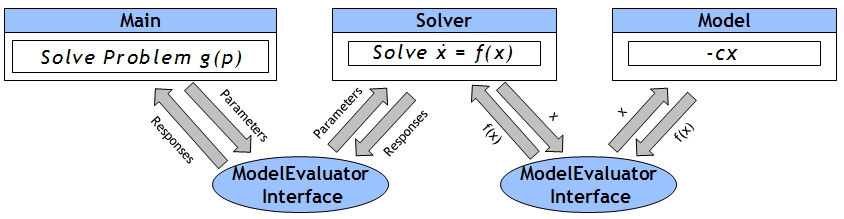
\includegraphics[width=\linewidth]{SimpleODEInterface}
 \end{center}
 \caption{Diagram of the control flow in \emph{SimpleODE}, showing two use cases of \emph{ModelEvaluator}. Execution begins with \texttt{main()}, which calls a \emph{ModelEvaluator}-wrapped Rythmos solver to solve an abstract problem $g(p)$. The Rythmos solver integrates an ODE in time, with the solver making calls to a separate \emph{ModelEvaluator}-wrapped model.}
\label{fig:SimpleODEInterface}
\end{figure}

The problem solved by \emph{SimpleODE} fits completely and naturally into the assumptions and contract enforced by the model evaluator interface, as the function $\mathbf{f}(x) = -c x$ is a pure mathematical function, and thus referentially transparent.

\subsection{\emph{Albany}, an Agile Components Demonstration and Prototype Code} \label{sec:albany}

The \emph{Albany} code is the original code designed to drive and demonstrate the Agile Components vision~\cite{AlbanyWebPage:2011}. \emph{Albany} serves as an early adopter and ripener of new algorithm libraries, a place to design and mature interfaces, and as a prototype \emph{Trilinos}-based application with a functioning software quality environment.

\emph{Trilinos}, in its role as a delivery vehicle for software libraries, has rapidly expanded beyond solvers to include numerous other computational science libraries. \emph{Albany} has helped mediate this growth by being an early adopter of many of these new capabilities. \emph{Albany} has been a place to mature the usability, robustness, flexibility, and scalability of these algorithms. It has also been a place to devise a larger domain model, so that the aggregate of capabilities does not have gaps or overlap.

A large fraction of the new capabilities vetted in \emph{Albany} are tailored to partial differential equations and finite element methods, and are not directly relevant to \emph{Peridigm}. However, the use of the model evaluator as the application abstraction (application abstract interface in Figure \ref{fig:ACAlbany}) occurred within \emph{Albany}, as did the wrapping of transient and nonlinear solvers (Rythmos and NOX) within this abstraction, as described in \S\ref{sec:simpleode}. Much of this work was concurrent with, and was influenced by, \emph{Peridigm} development.

In its role as a prototype code, \emph{Albany} has a small physics set as part of the main code base. This includes heat transfer, incompressible fluid flow, and a thermo-electrical model. These are meant to be sufficient for testing the full infrastructure (from input file parsing to uncertainty quantification). The embedded uncertainty quantification research program of Phipps uses \emph{Albany}, and these physics sets, to demonstrate and evaluate their algorithms. In addition, application-oriented projects have put physics sets within Albany. We describe those projects briefly in the following subsections.

\subsubsection{\emph{Albany} QCAD: Quantum Device Simulation Tool} \label{sec:albany:qcad}

The QCAD project is building a quantum device simulation tool within \emph{Albany}~\cite{QCADWebPage:2011}. The goal is to evaluate and design structures built from the tools of the semiconductor industry (doped semiconductors, oxide layers, gates) to isolate quantum dots. The primary computational science focus has been on development of a nonlinear Poisson solver to solve for the electrical potential in the device as a function of design and applied voltage. As a second step, a Schr\"{o}dinger solver has been developed and coupled to the nonlinear Poisson solver to capture quantum effects in the region of the device with few free electrons.

The QCAD application was an ideal fit for the current state of the Agile Components vision and the pieces already assembled and matured in the Albany infrastructure. The application's models are stateless, referentially transparent pure mathematical functions, satisfying the assumptions of the \emph{ModelEvaluator} interface. The application could make full use of the finite element mesh database, discretization algorithms, automatic differentiation technology, rapid insertion of new physics modules, nonlinear solvers, eigensolver, and optimization algorithms. As a result, this project is on its third-year milestones at the end of one year and is being used by customers as a production code. Much of the infrastructure improvements motivated by QCAD involve post-processing capabilities.  Many of these capabilities reside in \emph{Albany}, and some have migrated back to \emph{Trilinos} in terms of bug fixes and enhancements to the SIERRA toolkit (STK) and Sandia Engineering Analysis Code Access System (SEACAS) I/O tools.

\subsubsection{\emph{Albany} LCM: Computation Mechanics Research Code} \label{sec:albany:lcm}

The Laboratory for Computational Mechanics (LCM) project is creating a research and development platform for mechanics, particularly failure and fracture models~\cite{LCMWebPage:2011}. Its serves as a platform to rapidly and flexibly test new ideas and algorithms, with subsequent migration into associated production codes. As an open source code, it also serves as a vehicle for external collaborations.

The LCM is written as a (configure-time) physics set within the \emph{Albany} code. As with QCAD, the LCM project has made excellent progress in just one year, being an excellent fit with much of the finite-element based technology in \emph{Albany}. However, the LCM project also presents some of the same issues as the \emph{Peridigm} application, exposing assumptions or gaps in the current Agile Components instantiation. These include the potential statefulness of the model, where the current residual evaluation depends on the history and not just the current state. In the case of solid mechanics, this can be the residual stress field or a model for material damage. The LCM and \emph{Peridigm} projects have leveraged each other's experience in dealing with state data. As with \emph{Peridigm}, the time-dependent LCM applications are second order in time. One implicit and one explicit second-order time integrator have been written into the \emph{Trilinos} package Piro, but currently function only with a modified \emph{ModelEvaluator} interface.

\subsection{\emph{Peridigm}, A Peridynamics Code} \label{sec:peridigm}

The \emph{Peridigm} code, through consequence of its computational structure and material models, violates several assumptions of the \emph{ModelEvaluator} interface. We first discuss the mathematical formulation of the peridynamic equation of motion, followed by specific details of each development issue encountered, concluding with specific recommendations for future Agile Components development.

In the peridynamic theory, the deformation at a point depends collectively on all points interacting with that point. Using the notation of \cite{Silling:2007:PDStates}, we write the peridynamic equation of motion as
\begin{equation} \label{eqn:PDEOM}
\rho(\mathbf{x}) \ddot{\mathbf{u}}(\mathbf{x},t) = \int_{\mathcal{H}_{\mathbf{x}}}
\left\{ \underline{\mathbf{T}}\left[ \mathbf{x},t \right]\left<\mathbf{x}^{\prime}-\mathbf{x} \right>
 - \underline{\mathbf{T}}\left[\mathbf{x}^{\prime},t \right]\left<\mathbf{x}-\mathbf{x}^{\prime} \right> \right\}
{d}V_{\mathbf{x}^\prime} + \mathbf{b}(\mathbf{x},t),
\end{equation}
where $\rho$ represents the mass density, $\underline{\mathbf{T}}$ the force vector state, and $\mathbf{b}$ an external body force density. A point $\mathbf{x}$ interacts with all the points $\mathbf{x}^{\prime}$ within the neighborhood $\mathcal{H}_{\mathbf{x}}$, assumed to be a spherical region of radius $\delta>0$ centered at $\mathbf{x}$. $\delta$ is called the {\em horizon}, and is analogous to the cutoff radius used in molecular dynamics. For more on the peridynamic equation of motion, see see \cite{Silling:2007:PDStates}.

\emph{Peridigm} solves \eqref{eqn:PDEOM} with appropriate initial and boundary conditions. Based upon \emph{Trilinos} components, \emph{Peridigm} inherits standard software practices and tools used in \emph{Trilinos} development, some of which are depicted graphically in Figure \ref{fig:PeridigmComponents}. \emph{Peridigm} provides parallel simulation, peridynamic material models such as the linear peridynamic solid (LPS) model \cite{Silling:2007:PDStates}, a peridynamic plasticity model~\cite{Mitchell:2011:Plasticity}, and a peridynamic viscoelastic model. \emph{Peridigm} provides both explicit and implicit time integration.  A contact algorithm is available in the case of explicit time integration.  It has the capability to dynamically load balance running simulations to achieve better parallel performance. It is capable of reading Exodus meshes as input or internally generating meshes of simple geometric solids. Output is to VTK-format files. The user can define their own ``compute'' styles to output quantities of interest to them.

\begin{figure}[h!]
\begin{center}
	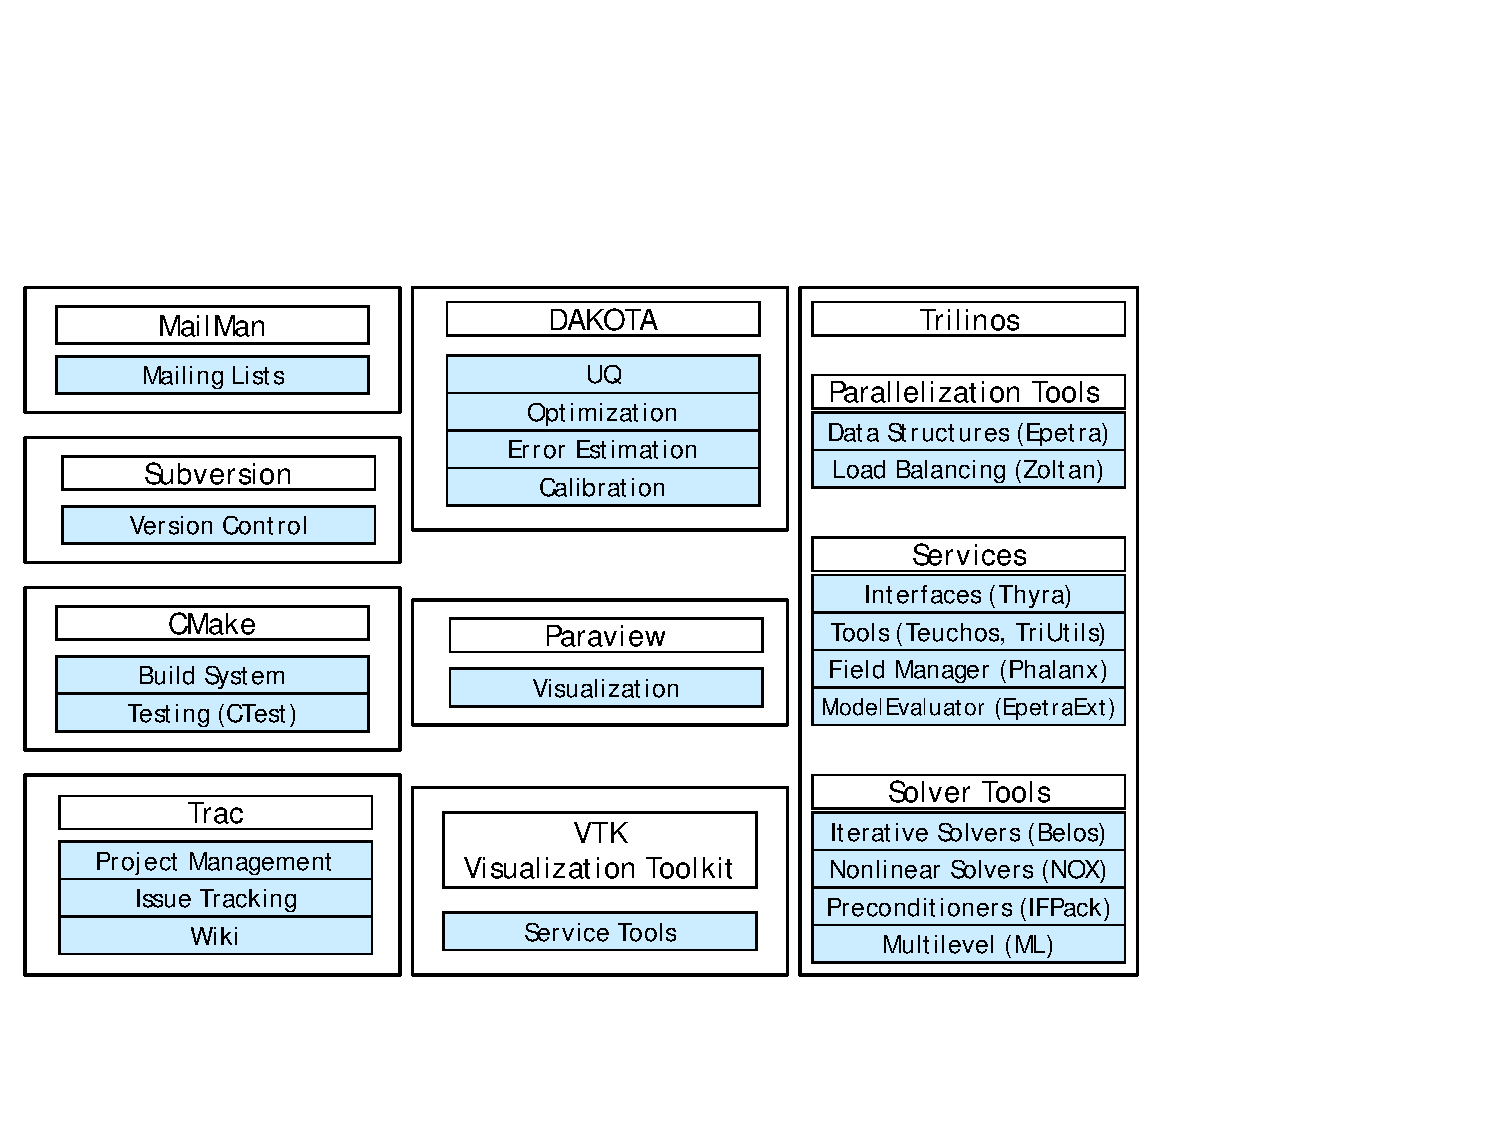
\includegraphics[width=\linewidth]{PeridigmComponents}
 \end{center}
 \caption{Graphical representation of the software components, interfaces, tools, and quality practices that comprise \emph{Peridigm}.}
\label{fig:PeridigmComponents}
\end{figure}

\begin{rem}
\textbf{Differences between peridynamics and PDE-based finite element models have motivated new development in Agile Components. Key driving factors were the need for history-dependant material models and load rebalance within \emph{Peridigm}.}
\end{rem}

\subsubsection{Handling Model State}

The \emph{ModelEvaluator} interface assumes stateless models. When implementing \emph{Peridigm}, we encountered two significant issues regarding the handling of model state. The first arises because many material models of interest contain state in the form of history dependence, and these models violate the assumption made by the \emph{ModelEvaluator} of a stateless model. The second issue was discovered when attempting to implement load rebalance. Each \emph{ModelEvaluator}-derived class creates and stores its own parallel data distribution across processors, which is a form of state data. This behavior is ostensibly in violation of the \emph{ModelEvaluator} contract that they be stateless. This only manifests as a problem when attempting to redistribute data across processors, which is necessary when performing either load rebalance, or mesh adaptivity.

\paragraph{History Dependence in Material Models}

Practical peridynamic material models contain state in the form of history dependence. This history dependence is not unique to peridynamics -- the majority of material models in practical computational solid mechanics applications are not stateless. Within \emph{Peridigm}, specifically, all models contain a fracture rule governing the breaking of peridynamic bonds, which is a history-dependent phenomenon. Additionally, \emph{Peridigm} also contains a peridynamic plasticity model, which uses history-dependent state~\cite{Mitchell:2011:Plasticity}.

To address the \emph{ModelEvaluator} assumption of statelessness, we utilized an \emph{observer} design pattern.
\begin{defn}
The observer pattern is a software design pattern in which an object (called the subject) maintains a list of its dependents (called observers) and notifies them of any state changes, usually by calling one of their methods.
\end{defn}
\noindent
Specifically, we implemented our material models as a \emph{ModelEvaluator}-derived class, storing the model state within the class. This is ostensibly a violation of the \emph{ModelEvaluator} contract, but does not manifest for explicit or implicit time integration. An observer was called from the time integrator to inform the material model that a time step had been completed, and that the material model should update its internal state.

While this approach is effective for time integration, it's not clear that this remedy would work for more complicated scenarios, such as adaptive time stepping or optimization.

\paragraph{Load Rebalance and Mesh Adaptivity}

Peridynamics is commonly used for modeling fragmentation problems, where material initially contained in a relatively small spatial region becomes spread over a much larger spatial region during the course of the simulation. In order to preserve parallel load balance, it is periodically necessary to redistribute data across processors. In the \emph{Trilinos} framework, data assignment to processors is encapsulated within a \emph{map} class, such as \texttt{Epetra::Map} or \texttt{Epetra::BlockMap}. To perform a rebalance, \emph{Peridigm} asks the Zoltan package to determine a near-optimal data distribution across processors in the current configuration, which can be used to determine a new map. Given the current map (containing the current data distribution across processors) and the new map (containing the desired data distribution across processors), an import/export operation can be called to migrate data between processors.

Mesh adaptivity, or adaptive mesh refinement, also involves redistributing data. During the course of a computation one may desire to adaptively refine a mesh, for example, to reduce error in localized regions of the computational domain. This dynamically introduces more degrees of freedom into the problem, necessitating that one migrate data from an old map (the coarse mesh) to a new map (the fine mesh).

Load rebalance and mesh adaptivity have proven problematic with the \emph{ModelEvaluator} interface. \emph{ModelEvaluator}-derived classes have the property that they produce their own input parameter and output response data structures, as can be seen in this code segment taken from \emph{SimpleODE}:
\begin{quote}
\vspace{-5pt}
\texttt{SimpleODE::SolverFactory slvrfctry(xml\_file\_name, appComm);}\\
\texttt{Teuchos::RCP<EpetraExt::ModelEvaluator> App = slvrfctry.create();}\\
\texttt{EpetraExt::ModelEvaluator::InArgs params\_in = App->createInArgs();}\\
\texttt{EpetraExt::ModelEvaluator::OutArgs responses\_out = App->createOutArgs();}\\
\vspace{-17pt}
\end{quote}
This behavior is beneficial in that it makes the model self-contained. However, each model makes its own maps and control its data distribution across processors, as seen here, where the ModelEvaluator-derived class ``App'' returns a map:
\begin{quote}
\vspace{-5pt}
\texttt{Teuchos::RCP<Epetra\_Vector> g}\\
\texttt{= Teuchos::rcp(new Epetra\_Vector(*App->get\_g\_map(0)));}\\
\vspace{-17pt}
\end{quote}
This property of \emph{ModelEvaluator}-derived classes presented an issue when trying to perform a rebalance with \emph{Peridigm}. The maps are a form of state data contained within the \emph{ModelEvaluator}-derived classes, ostensibly in violation of the \emph{ModelEvaluator} contract that they be stateless. Unlike the issue with history-dependant material models, discussion with other \emph{Trilinos} developers did not reveal a clear path forward. One idea proposed was to generate a ``meta-ModelEvaluator'' that would transform a \emph{ModelEvaluator}-derived class (using an old map) to a \emph{ModelEvaluator}-derived class (using a new map). This idea was not pursued as it would require a substantial coding effort, in part because each \emph{ModelEvaluator}-derived class would require an associated expert-developed meta-ModelEvaluator class to effect a rebalance. An alternative approach is to destroy the existing \emph{ModelEvaluator} objects, creating new ones in their place. This process is equivalent to the process that would need to occur, for example, if a simulation running on $N_1$ processors was checkpointed and then restarted on $N_2$ processors.

To overcome this obstacle and proceed with \emph{Peridigm} development, we instead developed a \emph{ModelEvaluator}-like class (\texttt{Peridigm::ModelEvaluator}) that mimics the interface of the \emph{ModelEvaluator} used in the Agile Components frameworks, but does not create its own maps. Instead, maps are created externally and passed into the \texttt{Peridigm::ModelEvaluator}.

\subsubsection{Data Distribution}

Another issues encountered during \emph{Peridigm} development was the requirement by the \emph{ModelEvaluator} interface that \texttt{Epetra::Map} and \texttt{Epetra::Vector} data structures be used, rather than the more general \texttt{Epetra::BlockMap} and \texttt{Epetra::MultiVector} data structures. In the Epetra inheritance diagrams, an \texttt{Epetra::Vector} inherits from an \texttt{Epetra::MultiVector}, and an \texttt{Epetra::Map} inherits from an \texttt{Epetra::BlockMap}, meaning that the block map and multivector data structures are more general.

In peridynamics, we frequently have multiple degrees of freedom per node (for example, all 3D vector fields have three degrees of freedom per node). The \texttt{Epetra::BlockMap} and \texttt{Epetra::MultiVector} data structures were designed for this use case, and are more natural to use within material model evaluation routines. To utilize the \emph{ModelEvaluator} interface, it was necessary to use the \texttt{Epetra::Vector} and \texttt{Epetra::Map} data structures, which required mapping from \texttt{Epetra::MultiVector}s to \texttt{Epetra::Vector}s and back every time step. Implementing this mapping was tedious and time-consuming, and impaired rapid code development. Additionally, in addition to requiring extra computation, this led to redundant data structures in the code (\emph{e.g.}, one \texttt{Epetra::BlockMap} and one or more \texttt{Epetra::Map}s for every given field variable).

\subsubsection{Time Integration}

When initially developing \emph{Peridigm}, we attempted to use Rythmos, the lone time integration package in \emph{Trilinos}. Unfortunately, none of the explicit integrators in Rythmos are for second-order ODEs, and all of the explicit integrators in Rythmos are unconditionally unstable when applied to the peridynamic equation of motion when it is reformulated as a first-order ODE. This is not a shortcoming of the Agile Components approach, but simply an observation that the solver tools needed by \emph{Peridigm} were not initially present in any \emph{Trilinos} package.

Motivated by the needs of \emph{Peridigm}, a second-order explicit integrator has been added to the Piro package within \emph{Trilinos}.

\subsubsection{Control Flow}

Another issue encountered during \emph{Peridigm} development was managing the execution control flow. The standard Agile Components approach is to cast the problem to be solved as a single \emph{ModelEvaluator} instance, and evaluate that model to return the solution. This is depicted in Figure \ref{fig:SimpleODEInterface}.

However, a standard expectation of developers of computational solid mechanics codes is that one has the ability to intervene and modify simulation data at arbitrary points during the simulation. As a practical example, it is standard practice to execute contact resolution algorithms between atomic steps of an explicit time integration algorithm to ensure that solids do not interpenetrate each other.

This issue lead to a reformulation of the control flow within \emph{Peridigm}. Originally mimicking the control flow of \emph{SimpleODE} in Figure \ref{fig:SimpleODEInterface}, the control flow of \emph{Peridigm} now has only one instance of a \emph{ModelEvaluator} object (that encapsulates the material model), and a \texttt{main()} routine that allows the simulation data to potentially be modified between atomic steps of time integration routines. The rationale for this decision is that it is not the providence of the material model nor the solver to perform tasks such as contact resolution or rebalance. Such tasks naturally fall to a \texttt{main()} routine, at the the highest level of control in the program.

\section{Other Remarks}

The \emph{Phalanx} package for evaluating field variables was among the more recently developed \emph{Trilinos} components utilized in \emph{Peridigm}~\cite{PhalanxWebPage:2011}.  \emph{Phalanx} was integrated within \emph{Peridigm} with no significant stumbling blocks, and was found to be an effective tool for managing field evaluators.  We expect this is the case because Phalanx was developed based on practical experience gained from the \emph{Charon} and \emph{Aria} codes. Feedback from production codes into new software components provides a highly effective mechanism for immediately delivering mature capability.

%%% ----------------------------------------------------------------------
\section{Recommendations} \label{sec:recommendations}
Although some development issues were encountered deploying the Agile Components methodology in \emph{Peridigm}, we are supportive of the goals of Agile Components and view this report as an opportunity to further broaden the scope of applications suitable for use in the Agile Components framework. For models satisfying the assumptions of the \emph{ModelEvaluator} interface, the Agile Components methodology has proven to facilitate rapid development of powerful application code. For applications outside these target use cases, the potential rapid development capabilities that Agile Components may provide are simply too tantalizing to overlook. To that end, we make the following recommendations which we feel will strengthen the impact of Agile Components, and broaden its scope to new applications.

\begin{description}
  \item[Documentation] Attempting to learn the Agile Components methodology by reading \emph{Albany} code is somewhat like drinking from a fire hydrant. Although Agile Components developers are always happy to explain any concept, this approach is not scalable if we want the Agile Components methodology to be widely adopted beyond the current expert users. We recommend improved documentation along with an easy-to-understand demonstration code, such as \emph{SimpleODE}. This will greatly shorten the learning curve for new users, and help them to understand how their application fits within the Agile Components methodology. \emph{SimpleODE} may be useful as a starting template for new users to develop their own application based upon Agile Components.
  \item[Graceful Handling of Model State] We recommend that all service modules, such as \emph{ModelEvaluator}-derived classes, be made referentially transparent (\emph{c.f.} Defn. \ref{defn:RT}). This would eliminate any and all issues with regard to rebalance and mesh adaptivity, the biggest obstacles encountered. The consequence of this is that \emph{ModelEvaluator}-derived classes must no longer allocate their own maps, data structures, etc., but that these must be passed in externally. Referring to the control flow diagram of Figure \ref{fig:SimpleODEInterface}, it is not the role of the mathematical model $\mathbf{f}$ nor of the solver to create these data structures, meaning that they must be created at the level of \texttt{main()} (by the application developer) and passed in. This requires a mechanism for the developer to gracefully and naturally hand in model state as input, have the \emph{ModelEvaluator} class potentially transform that state, and then hand that state back out. The \emph{ModelEvaluator} becomes less self-contained, but at the benefit of increased usability and flexibility. This recommendation comes at the cost of a substantial refactor of all agile component based code, and may not be feasible.
  \item[Data Distribution] If possible, we recommend moving the \emph{ModelEvaluator} interface and \emph{ModelEvaluator}-derived solvers to support BlockMap and MultiVector data structures. A Map is a special case of a BlockMap, and a Vector is special case of a MultiVector, so this would not impact any current use cases.
  \item[Control Flow] The control flow of Figure \ref{fig:SimpleODEInterface} could be preserved so long as the application developer has the opportunity and freedom to intervene during solver execution and modify simulation data in essentially arbitrary ways. One way to achieve this is by inserting callbacks between atomic steps in all \emph{ModelEvaluator}-derived solvers. The application developer would then have complete freedom to specify how simulation data should be transformed between atomic solver steps, without the solver itself ever having to know anything about contact resolution, rebalance, etc.\footnote{Such use of callbacks is common practice within Sandia's LAMMPS molecular dynamics code \cite{Plimpton:LAMMPS:1995}. The code makes callbacks to user-defined functions between atomic steps in time integration or minimization processes, and has been used to great effect.} For a specific example, see Algorithm \ref{alg:vel_verlet}, showing callbacks put in between steps of the velocity Verlet explicit time integrator.\footnote{This is exactly the callback structure used in LAMMPS.}
\end{description}

\begin{algorithm}
\caption{Velocity Verlet with Callbacks} \label{alg:vel_verlet}
\begin{algorithmic}[1]
   \STATE initial\_integrate()
   \STATE $\bdv_i^{n + 1/2} = \bdv_i^n + \frac{\Delta t}{2 \rho_i} \bdf_i^n$
   \STATE $\bdy_i^{n+1}     = \bdy_i^n + \Delta t \bdv_i^{n + 1/2}$
   \STATE post\_force()
   \STATE $\bdv_i^{n+1} = \bdv_i^{n+1/2} + \frac{\Delta t}{2 \rho_i} \bdf_i^{n+1}$
   \STATE final\_integrate()
\end{algorithmic}
\end{algorithm}

    \nocite{*}


    % ---------------------------------------------------------------------- %
    % References
    %
    \clearpage
    % If hyperref is included, then \phantomsection is already defined.
    % If not, we need to define it.
    \providecommand*{\phantomsection}{}
    \phantomsection
    \addcontentsline{toc}{chapter}{References}
    \bibliographystyle{plain}
    \bibliography{PeridigmFinalReport}


    % ---------------------------------------------------------------------- %
    %
%    \appendix
%    \chapter{Historical Perspective}
%    \chapter{Some Other Appendix}


    % \printindex

    %
% This is an example of how to create the distribution page. Some
% distributions are required by Sandia; e.g. the housekeeping copies.
% Depending on the type of report; e.g. CRADA, Patent Caution, etc.
% additional distribution lines may have to be added. See the
% "Guide for Preparing SAND Reports"
%
% SANDdistribution takes CA or NM as an optional argument. If given,
% the approrpiate housekeeping copies are inserted autmatically.
% Inside the SANDdistribution environment, several commands can be used
% insert the distributions for CRADA, LDRD, etc. See example below.
%
% You can leave the CA or NM option off and not use any of the SANDdist*
% commands. This will allow you to create a distribution list manually.
%
\begin{SANDdistribution}[NM]
    % Housekeeping copies necessary for every unclassified report:
    % \SANDdistCRADA	% If this report is about CRADA work
    % \SANDdistPatent	% If this report has a Patent Caution or Patent Interest
    % \SANDdistLDRD	% If this report is about LDRD work

    % The following MUST BE between the external and internal distributions!
    % \SANDdistClassified % If this report is classified

    % Internal Addresses
    \SANDdistInternal{1}{1322}{John Aidun}{1425}
    \SANDdistInternal{1}{1320}{Scott Collis}{1442}
    \SANDdistInternal{1}{0372}{Eliot Fang}{1524}
    \SANDdistInternal{1}{0372}{Mike Glass}{1545}
    \SANDdistInternal{1}{1318}{Bruce Hendrickson}{1440}    
    \SANDdistInternal{1}{1318}{Robert Hoekstra}{1426}    
    \SANDdistInternal{1}{0380}{Joe Jung}{1542}
    \SANDdistInternal{1}{0825}{Joel Lash}{1510}
    \SANDdistInternal{1}{1322}{David Littlewood}{1444}
    \SANDdistInternal{1}{1322}{John Mitchell}{1444}
    \SANDdistInternal{1}{1322}{Rick Muller}{1425}    
    \SANDdistInternal{1}{0316}{Larry Musson}{1425}
    \SANDdistInternal{1}{1320}{Michael Parks}{1444}
    \SANDdistInternal{1}{1318}{Roger Pawlowski}{1444}
    \SANDdistInternal{1}{1318}{Eric Phipps}{1441}    
    \SANDdistInternal{1}{9042}{Jake Ostien}{8246}
    \SANDdistInternal{1}{1318}{Andy Salinger}{1442}
    \SANDdistInternal{1}{1321}{Randall Summers}{1444}
    \SANDdistInternal{1}{0380}{David Womble}{1540}

    % Example of a mail channel use (instead of a mail stop)
%    \SANDdistInternalM{1}{M9999}{Someone}{01234}

\end{SANDdistribution}



\end{document}
